\documentclass[11pt]{article}
\usepackage{preamble}

\usepackage{listings, courier}
\lstset{basicstyle=\small\ttfamily,breaklines=true}
%mathtools included in preamble
\DeclarePairedDelimiter\ceil{\lceil}{\rceil}
\DeclarePairedDelimiter\floor{\lfloor}{\rfloor}


\titleformat*{\section}{\Large\bfseries}

\title{CISC 3220 Homework Chapter 7}
\author{Rachel Friedman}
\date{April 19, 2020}

\begin{document}
\maketitle

\section*{Exercise 7.1}\nointerlineskip
\noindent \rule{\linewidth}{0.01pt}\\

\subsubsection*{Question 7.1-1}\nointerlineskip

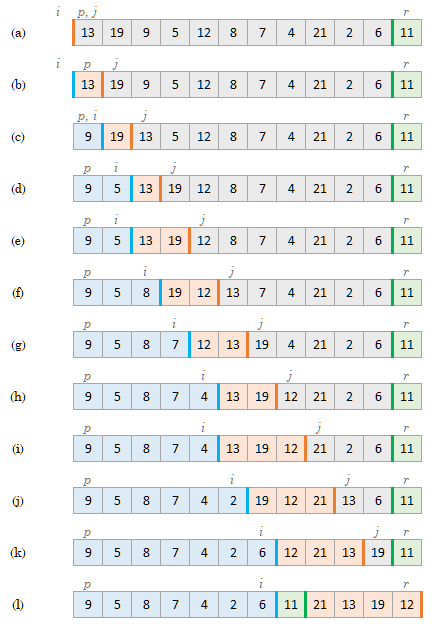
\includegraphics[scale=.9]{Ques_7-1-1.png}\\

\subsubsection*{Question 7.1-4}\nointerlineskip

To modify QUICKSORT to sort into nonincreasing order, change the algorithm to check if the element in position $j$ is \textbf{greater} than or equal to the pivot element:
\begin{center}  
\begin{minipage}{3in}
\begin{lstlisting}
if A[j] >= A[r]
\end{lstlisting}
\end{minipage}
\end{center}

\vspace{20pt}


\section*{Excercise 7.2}\nointerlineskip
\noindent \rule{\linewidth}{0.01pt}\\

\subsubsection*{Question 7.2-3}\nointerlineskip
Show that the running time of QUICKSORT is $\Theta(n^2)$ when the array $A$ contains distinct elements and is sorted in decreasing order.\\

Refer to this part of the Quicksort Algorithm:
\begin{center}  
\begin{minipage}{3in}
\begin{lstlisting}
QuickSort(A, p, r):
    if p < r:
        q = Partition(A, p, r)
        QuickSort(A, p, q - 1)
        QuickSort(A, q + 1, r)
\end{lstlisting}
\end{minipage}
\end{center}



In an array of decreasing order, the pivot element is smaller than all the other elements in the array. Thus, after the call to:  q = Partition(A, p, r), the pivot element is moved to the first position, and so $q=1$. Then, the the next two recursive Quicksort calls resolve as follows:
\begin{center}  
\begin{minipage}{4in}
\begin{lstlisting}
QuickSort(A,p,q-1) --> QuickSort(A,1,0)
QuickSort(A,q+1,r) --> QuickSort(A,2,r)
\end{lstlisting}
\end{minipage}
\end{center}

The resulting subarrays are of size 0 and of size $n-1$. The runtime of Partion is $\Theta(n)$. Therefore, the recurrence is:\\
\begin{flalign*}
T(n) &= T(0) + T(n-1) + \Theta(n)\\
&= T(n-1) + \Theta(n)\\
&= \Theta(n^2) \\
\end{flalign*}



\newpage
\section*{Exercise 7.3}\nointerlineskip
\noindent \rule{\linewidth}{0.01pt}\\

\subsubsection*{Question 7.3-2}\nointerlineskip
When RANDOMIZED-QUICKSORT runs, how many calls are made to the random-number generator RANDOM in the worst case? How about in the best case?\\

The RANDOMIZED-QUICKSORT function calls RANDOMIZED-PARTITION once, which then calls RANDOM once to pick the random number to be used as the pivot element. Therefore, the running time of this portion is $\Theta(1)$ (used below).\\

\textbf{Worst case scenario} occurs when partitioning results in one subarray of size 0 and one subarray of size $n-1$. The recurrence for that is:
\begin{flalign*}
T(n) &= T(0) + T(n-1) + \Theta(1) \\
&= T(n-1) + \Theta(1)\\
&= \Theta(n) \\
\end{flalign*}

\textbf{Best case scenario} occurs when partitioning results in two subarrays of size at most $n/2$. The recurrence for that is:
\begin{flalign*}
T(n) &= 2T(n/2) + \Theta(1)\\
&= \Theta(n) \textit{    By case 1 of the Master Theorem}\\
\end{flalign*}



\end{document}